\section{Asynchronous Completion Token}
\label{sec:asynchronous-completion-token}

The Asynchronous Completion Token design pattern allows an application to demultiplex and process efficiently the responses of asynchronous operations it invokes on services.

\subsection{Kontext}
Ein Event-gesteuertes System in welchem Applikationen asynchrone Operationen auf Diensten aufrufen und nach der Komplettierung die (natürlich asynchron eintreffenden) Event Responses verarbeiten.


\subsubsection*{Terminologie}

\begin{itemize}
	\item Service (Dienst) stellt eine Funktionalität zur Verfügung, welcher asynchron angesprochen werden kann
	\item Client Initiator (oder auch Applikation, Client Applikation) ruft asynchron Operationen auf einem Service auf
	\item Ein Asynchchrones Completion Token (ACT) beinhaltet Informationen über den Completion Handler des Initiators.
	\begin{itemize}
		\item Der Initiator gibt dieses ACT dem Dienst beim asynchronen Aufruf der Operation mit.
		\item Der Initiator verwendet dieses ACT nach der Response der asynchronen Operation um den richtigen Handler aufzurufen
	\end{itemize}
\end{itemize}


\subsection{Problem}

Wenn eine Applikation mehrere asynchrone Operationen ausführt, wird jeder Dienst die Antwort an die Applikation zurückgeben. Um die Komplettierungs-Events korrekt verarbeiten zu können, muss die Applikation die Events demultiplexen und somit zum richtigen Handler weiterleiten.
Drei Faktoren sind dabei wichtig und müssen gelöst werden:

\begin{itemize}
	\item Ein Dienst könnte den ursprünglichen Kontext, in welchem die Operation gestartet wurde, nicht kennen
	\item Um zu entscheiden wie die Applikation einen Completion Event demultiplexen und verarbeiten soll, soll so wenig Kommunikation wie möglich zwischen Applikation und Dienst ausgetauscht werden
	\item Sobald die Antwort eines Services bei der Client Applikation ankommt, soll so wenig Zeit wie möglich genutzt werden um den Beendigungs-Event zum Handler weiterzureichen
\end{itemize}


\subsection{Lösung}

Zusätzlich zu den normalen Informationen über den Event werden auch noch Daten mitgegeben, welche dem Initiator mitteilen, wie dieser den Event weiterverarbeiten soll.

\begin{figure}[H]
	\centering
	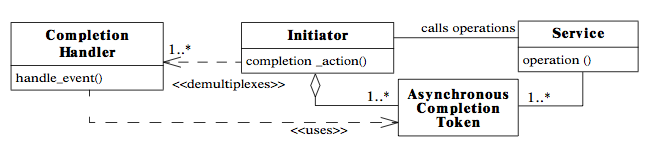
\includegraphics[width=12cm]{content/posa2/asynchronous-completion-token/images/class-diagram.png}
	\caption{Asynchronous Completion Token Klassendiagramm}
\end{figure}



\begin{figure}[H]
	\centering
	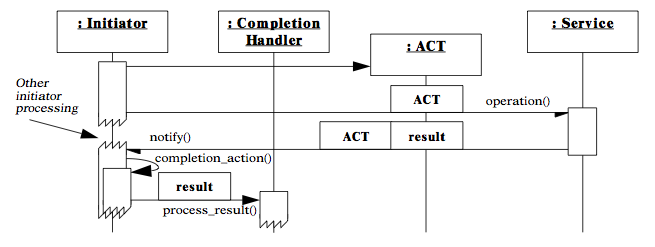
\includegraphics[width=12cm]{content/posa2/asynchronous-completion-token/images/ssd.png}
	\caption{Asynchronous Completion Token Sequenzdiagramm}
\end{figure}


\subsection{Varianten}

\begin{itemize}
	\item Chain of Service ACTs
	\begin{itemize}
		\item wenn Dienste ebenfalls die Rolle eines Initiators einnehmen, um asynchrone Operationen auf weiteren Services aufzurufen
		\item Chain of Services muss entscheiden, welcher Service dem ursprünglichen Initiator antwortet
		\item wenn keine zusätzlichen ACTs generiert werden, kann der letzte Service direkt dem Client antworten
		\item falls weitere ACTs generiert werden, muss die Sequenz korrekt eingehalten werden
	\end{itemize}
	\item Non-Opaque ACTs
	\begin{itemize}
		\item in manchen Implementationen ist die ACT mehr oder weniger transparent und kann verändert werden (u.a. Win32 OVERLAPPED Struktur)
	\end{itemize}
	\item Synchronous ACTs
	\begin{itemize}
		\item ACTs können auch für synchrone Callbacks verwendet werden
		\item Somit ist das Token mehr synchron als asynchron
		\item Der selbe Mechanismus zu verwenden garantiert aber eine gut strukturierte Art den Zustand eines Systems anderen Operationen/Diensten weiterzugeben
	\end{itemize}
\end{itemize}


\subsection{Verwendung}
\begin{itemize}
	\item AJAX
	\item JSONP
\end{itemize}


\subsection{Vorteile}

\begin{itemize}
	\item Initiator muss keine komplexen Datenstrukturen unterhalten, um die Antworten des Services mit den Completion Handler zu verknüpfen. ACT kann beispielsweise ein Pointer auf einen Completion Handler sein.
	\item ACTs sind flexibel und müssen kein bestimmtes Interface implementieren.
\end{itemize}

\subsection{Nachteile}

\begin{itemize}
	\item Wenn Pointer als ACTs verwendet werden, kann das zu Memory Leaks führen, wenn der entsprechende Callback nie kommt.
	\item Initiator muss dem Service vertrauen: ACT könnte bösartig sein (gerade im Falle des Pointers)
\end{itemize}


\subsection{Prüfungsfragen}

\begin{itemize}
	\item Was muss beim Dienst beachtet werden, wenn die aufgerufene asynchrone Methode selber auch asynchron abläuft?
	\begin{itemize}
		\item ACT muss in einer externen Datenstruktur gespeichert werden.
		\item Beim synchronen ablaufen der Methode könnte es auch einfach in der Run-time gespeichert werden.
	\end{itemize}
\end{itemize}
